\subsection{Construction: DFA Symbolic Finite Automata}

{  \setbeamercolor{background canvas}{bg=sectioncolor}
\begin{frame}{\Challenge{3} DFA Construction}

  Given an RTE, generate a finite automaton.

  \begin{itemize}
  \item Well-known techniques exists to construct DFAs from classical REs
    \begin{itemize}
      \item Brzozowski Derivative
  \end{itemize}
  \item Adapt them to work with RTEs
  \item Enforce determinism
  \end{itemize}
\end{frame}
}



\begin{frame}<0>{Demo}{Sample Flow}
   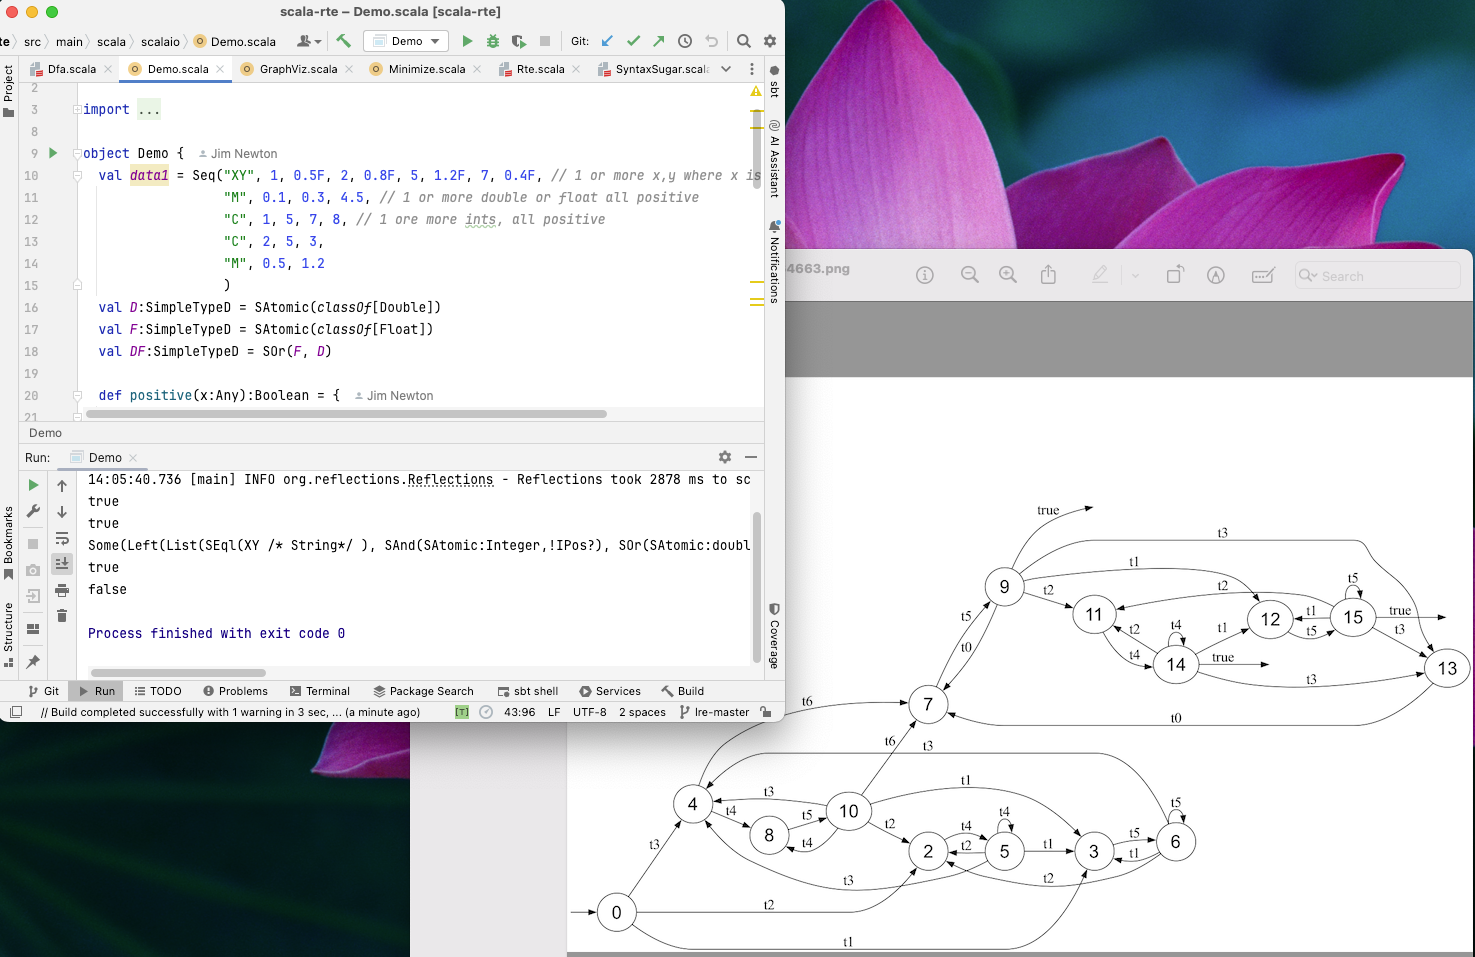
\includegraphics[height=0.8\textheight]{demo.png}
\end{frame}

\begin{frame}{RTE Construction}
  \begin{columns}
    \begin{column}{0.5\textwidth}
      How to construct the DFA corresponding to \[p_0=(int \cdot str^{*} \cdot even)^{*}\,.\]
      
      \includegraphics[width=0.9\textwidth,trim={1.4cm 1.2cm 1.4cm 0.8cm},clip=true]{reclojure-2025-sink-example-2}
    \end{column}
    \begin{column}{0.5\textwidth}
      \begin{align*}
        t_1 &= \Sigma\\
        t_2 &= int  \\
        t_3 &= \compl{int}\\
        t_4 &= str \cap even\\
        t_5 &= \compl{str} \cap even\\
        t_6 &= str \cap \compl{even}\\
        t_7 &= (int \cap \compl{even}) \cup (str \cap \compl{even})\\
        t_8   &=\compl{int} \cap \compl{str} \cap even\\
        t_9 &=(int \cap even) \cup (str \cap even)\\
        t_{10} &=\compl{str} \cap \compl{even}\\
        t_{11} &=\compl{int} \cap \compl{str} \cap \compl{even}
      \end{align*}
    \end{column}
  \end{columns}
\end{frame}


\newsavebox\boxa
\begin{lrbox}{\boxa}
  \begin{minipage}{0.4\textwidth}
\begin{align*}
  \deriv{\typevar}{(r^{*})}      &= (\deriv{\typevar}{r}) \cdot r^{*}\\
  \deriv{\typevar}{(r \reor s)}   &= \deriv{\typevar}{r} ~ \reor~ \deriv{\typevar}{s}\\
  \deriv{\typevar}{(r \reand s)} &= \deriv{\typevar}{r} ~ \reand~  \deriv{\typevar}{s}\\
  \deriv{\typevar}{(r\!\cdot\! s)} & =\! \begin{cases}
    \!(\deriv{\typevar}{r})\cdot s & \text{if $()\!\not\in\!\sem{r}$} \\
    \!(\deriv{\typevar}{r})\cdot s \reor \deriv{\typevar}{s} & \text{if $()\!\in\!\sem{r}$}
  \end{cases}\\
  \deriv{\typevar}{\!\renot{r}}  &= \renot{\deriv{\typevar}{r}}
\end{align*}
  \end{minipage}
\end{lrbox}



\newsavebox\boxb
\begin{lrbox}{\boxb}
  \begin{minipage}{0.55\textwidth}
\begin{align*}
  \deriv{\typevar}{\emptyset}  &=\emptyset\\
  \deriv{\typevar}{\varepsilon} &=\emptyset\\
  \deriv{\typevar}{\singleton{\typevart}} &= \varepsilon \quad \text{ if } \sem{\typevar} \subseteq \sem{\typevart} \\
  \deriv{\typevar}{\singleton{\typevart}} &= \emptyset \quad \text{ if } \sem{\typevar} \setand \sem{\typevart}=\emptyset         \\
  \deriv{\typevar}{\singleton{\typevart}} &\quad   \text{ otherwise, no rule defined}   
\end{align*}
  \end{minipage}
\end{lrbox}



\begin{frame}{RTE Construct}

\only<1,2,3>{{\LARGE
  Brzozowski Derivative: $\deriv{\typevar}{r}$
  }

  \medskip
  }
\only<1>{%
\quad\quad$\begin{cases}r,s~ &\text{designate  RTEs}\\\typevar, \typevart ~&\text{designate types}\end{cases}$.
  \quad\quad\Eg, $\begin{cases}r&=(int \cdot str^{*} \cdot even)^{*}\\ \typevar&=\tyint\end{cases}$.

\medskip

\begin{tabular}{c|c}
  \textbf{Recursive Rules}&\textbf{Terminal Rules}\\
  \hline
  \usebox\boxa & \usebox\boxb
\end{tabular}
}%
\only<2>{%
  \begin{align*}
  \deriv{\typevar}{\singleton{\typevart}} &= \varepsilon \quad \text{ if } \sem{\typevar} \subseteq \sem{\typevart} \\
  \deriv{\typevar}{\singleton{\typevart}} &= \emptyset \quad \text{ if } \sem{\typevar} \setand \sem{\typevart}=\emptyset         \\
  \deriv{\typevar}{\singleton{\typevart}} &\quad   \text{ otherwise, no rule defined}   
  \end{align*}
  }%
\only<3>{%
  \begin{align*}
  \deriv{\typevar}{\singleton{\typevart}} &= \varepsilon \quad \text{ if } \sem{\typevar} \subseteq \sem{\typevart} \\
  \deriv{\typevar}{\singleton{\typevart}} &= \emptyset \quad \text{ if } \sem{\typevar} \subseteq \setnot{\sem{\typevart}}         \\
  \deriv{\typevar}{\singleton{\typevart}} &\quad   \text{ otherwise, no rule defined}   
  \end{align*}

  \textcolor{red}{Houston we have a problem:} The subtype relation is \Emph{sometimes unknowable}.

  \Challenge{4} How to \Emph{sufficiently} partition types to assure $\deriv{\typevar}{\singleton{\typevart}}$ is computable?
}%
\end{frame}

\begin{frame}{      State Construction by   Brzozowski Derivative}
  \begin{columns}
    \begin{column}{0.4\textwidth}
      Compute RTEs:
      \[\{\deriv{\typevar}{p_0} \mid \typevar \in MDTD(1sts(p_0))\}\]

      1:1 correspondence state to unique RTE
    \end{column}
    \begin{column}{0.6\textwidth}
      \scalebox{0.8}{\documentclass{standalone}
  \usepackage{tikz}
  \usetikzlibrary{arrows.meta, automata, bending, positioning, shapes.misc}
  \tikzstyle{automaton}=[shorten >=1pt, >={Stealth[bend,round]}, initial text=]
  \tikzstyle{accepting}=[double]

\begin{document}
\begin{tikzpicture}[automaton, auto, thick]
  \node[state,initial,rounded rectangle] (0) {$p_0$};
  \node[state,rounded rectangle] (1) [above right=20mm and 50mm of 0] {$p_1 = \deriv{\typevar_1}{p_0}$};
  \node[state,rounded rectangle] (2) [right=50mm of 0] {$p_2 = \deriv{\typevar_2}{p_0}$};
  \node[state,rounded rectangle] (3) [below right=20mm and 50mm of 0] {$p_3 = \deriv{\typevar_3}{p_0}$};

  \path[->] (0) edge[line width=2pt] node {$\typevar_1$} (1);
  \path[->] (0) edge[line width=2pt] node {$\typevar_2$} (2);
  \path[->] (0) edge[swap,line width=2pt]  node[pos=.5] {$\typevar_3 \ldots$} (3);
\end{tikzpicture}
\end{document}
}%
    \end{column}
  \end{columns}
\end{frame}


\begin{frame}{RTE Construction of \nodecirc{$p_0$}}
  \begin{columns}
    \begin{column}{0.45\textwidth}
      Step 1: construct transitions from~\nodecirc{$p_0$} using Brzozowski derivatives of RTE~$p_0$.

      \[p_0=(int \cdot str^{*} \cdot even)^{*}\,.\]


      \only<1-2>{\includegraphics[width=0.9\textwidth,trim={1.4cm 1.2cm 1.4cm 0.8cm},clip=true]{reclojure-2025-sink-example-pre}}%
      \only<3>{\includegraphics[width=0.9\textwidth,trim={1.4cm 1.2cm 1.4cm 0.8cm},clip=true]{reclojure-2025-sink-example-pre-p1}}%
      \only<4->{\includegraphics[width=0.9\textwidth,trim={1.4cm 1.2cm 1.4cm 0.8cm},clip=true]{reclojure-2025-sink-example-p0}}
    \end{column}
    \begin{column}{0.55\textwidth}
      \begin{itemize}
      \item<1->{What are the \emph{first} types of $p_0$: $\{\tyint\}$.}
      \item<2->{Partition $\Sigma$ by $\{\tyint\} \to \{\tyint,\tynot{\tyint}\}$.}
      \item<3->{$\deriv{\tynot{\tyint}}{p_0} = \underbrace{\emptyset}_{p_1}$}
      \item<4->{$\deriv{\tyint}{p_0} = \underbrace{\tystring^{*} \cdot \tyeven \cdot (\tyint \cdot \tystring^{*} \cdot \tyeven)^{*}}_{p_2}$}
      \end{itemize}
    \end{column}
  \end{columns}
\end{frame}

\begin{frame}{RTE Construction  of \nodecirc{$p_0$}}
  \begin{columns}
    \begin{column}{0.5\textwidth}
      \includegraphics[width=0.9\textwidth,trim={1.4cm 1.2cm 1.4cm 0.8cm},clip=true]{reclojure-2025-sink-example-p0}

      \begin{align*}
        p_0 &= (int \cdot str^{*} \cdot even)^{*}\\
        p_1 &= \deriv{\tynot{\tyint}}{p_0} = \emptyset\\
        p_2 &= \deriv{\tyint}{p_0}    
        = \tystring^{*} \cdot \tyeven \cdot (\tyint \cdot \tystring^{*} \cdot \tyeven)^{*}
      \end{align*}

    \end{column}
    \begin{column}{0.5\textwidth}
      \begin{align*}
        t_2 &= \tyint  \\
        t_3 &= \compl{\tyint}
      \end{align*}
    \end{column}
  \end{columns}
\end{frame}

\begin{frame}{RTE Construction of \nodecirc{$p_1$}}
  \begin{columns}
    \begin{column}{0.45\textwidth}
      Step 2: construct transitions from~\nodecirc{$p_1$} using Brzozowski derivatives of RTE~$p_1$.

      \[p_1=\emptyset\,.\]

      \includegraphics[width=0.9\textwidth,trim={1.4cm 1.2cm 1.4cm 0.8cm},clip=true]{reclojure-2025-sink-example-p1}
    \end{column}
    \begin{column}{0.55\textwidth}
      \begin{itemize}
      \item<1->{What are the \emph{first} types of $p_1$: $\{\emptyset\}$.}
      \item<2->{Partition $\Sigma$ by $\{\emptyset\} \to \{\Sigma\}$.}
      \item<3->{$\deriv{\Sigma}{\emptyset} = \emptyset$}
      \item<4->{      \begin{align*}
        t_1 &= \Sigma\\
        t_2 &= \tyint  \\
        t_3 &= \compl{\tyint}
      \end{align*}}
      \end{itemize}
    \end{column}
  \end{columns}
\end{frame}



\begin{frame}{RTE Construction of \nodecirc{$p_2$}}
  \begin{columns}
    \begin{column}{0.45\textwidth}
      Step 3: construct transitions from~\nodecirc{$p_2$}: compute Brzozowski derivatives of 
      \[p_2=\tystring^{*}\cdot \tyeven \cdot(\tyint \cdot \tystring^{*} \cdot \tyeven)^{*}\,.\]

      \only<1-2>{\includegraphics[width=0.9\textwidth,trim={1.4cm 1.2cm 1.4cm 0.8cm},clip=true]{reclojure-2025-sink-example-p1}}%
      \only<3>{\includegraphics[width=0.9\textwidth,trim={1.4cm 1.2cm 1.4cm 0.8cm},clip=true]{reclojure-2025-sink-example-p2}}
    \end{column}
    \begin{column}{0.55\textwidth}
      \begin{itemize}
      \item<1->{What are the \emph{first} types of $p_2$: $\{\tystring,\tyeven\}$.}
      \item<2->{Partition $\Sigma$ by $\{\tystring,\tyeven\} \to \Pi$.}
      \item<3->{For each $\typevar \in \Pi$ compute $\deriv{\typevar}{p_2}$
        \begin{itemize}
        \item $\deriv{\tystring\cap\tyeven}{p_2} = p_3$ (NEW)
        \item $\deriv{\tystring\cap\tynot{\tyeven}}{p_2} = p_2$
        \item $\deriv{\tynot{\tystring}\cap\tyeven}{p_2} = p_0$
        \item $\deriv{\tynot{\tystring}\cap\tynot{\tyeven}}{p_2} = p_1$
        \end{itemize}
      }
      \end{itemize}
    \end{column}
  \end{columns}
\end{frame}

\begin{frame}{RTE Construction  of \nodecirc{$p_2$}}
  \begin{columns}
    \begin{column}{0.5\textwidth}
      \includegraphics[width=0.9\textwidth,trim={1.4cm 1.2cm 1.4cm 0.8cm},clip=true]{reclojure-2025-sink-example-p2}

      \begin{align*}
        p_0 &= (int \cdot str^{*} \cdot even)^{*}\\
        p_1 &= \emptyset\\
        p_2 &= \tystring^{*} \cdot \tyeven \cdot (\tyint \cdot \tystring^{*} \cdot \tyeven)^{*}\\
        p_3 &= \tystring^{*}\!\!\cdot\! \tyeven\!\cdot\! (\tyint\! \cdot\! \tystring^{*}\!\!\cdot\! \tyeven)^{*}\\
        &\quad\quad\reor (\tyint\! \cdot\! \tystring^{*}\!\!\cdot\!\! \tyeven)^{*}
      \end{align*}

    \end{column}
    \begin{column}{0.5\textwidth}
      \begin{align*}
        t_1 &= \Sigma\\
        t_2 &= \tyint  \\
        t_3 &= \compl{\tyint}\\
        t_4 &= \tystring \cap \tyeven\\
        t_5 &= \compl{\tystring} \cap \tyeven\\
        t_6 &= \tystring \cap \compl{\tyeven}\\
        %%t_7 &= (\tyint \cap \compl{\tyeven}) \cup (\tystring \cap \compl{\tyeven})\\
        %%t_8 &=\compl{\tyint} \cap \compl{\tystring} \cap \tyeven\\
        %%t_9 &=(\tyint \cap \tyeven) \cup (\tystring \cap \tyeven)\\
        t_{10} &=\compl{str} \cap \compl{even}\\
        %%t_{11} &=\compl{int} \cap \compl{str} \cap \compl{even}
      \end{align*}
    \end{column}
  \end{columns}
\end{frame}




\begin{frame}{RTE Construction of \nodecirc{$p_3$}}
  \begin{columns}
    \begin{column}{0.45\textwidth}
      Step 4: construct transitions from~\nodecirc{$p_3$}: compute Brzozowski derivatives of 
      \begin{align*}
        p_3&=\tystring^{*}\!\!\cdot\! \tyeven\!\cdot\! (\tyint\! \cdot\! \tystring^{*}\!\!\cdot\! \tyeven)^{*}\\
        &\quad\quad\reor (\tyint\! \cdot\! \tystring^{*}\!\!\cdot\!\! \tyeven)^{*}
      \end{align*}
      \only<1-2>{\includegraphics[width=0.9\textwidth,trim={1.4cm 1.2cm 1.4cm 0.8cm},clip=true]{reclojure-2025-sink-example-p2}}%
      \only<3->{\includegraphics[width=0.9\textwidth,trim={1.4cm 1.2cm 1.4cm 0.8cm},clip=true]{reclojure-2025-sink-example-2}}
    \end{column}
    \begin{column}{0.55\textwidth}
      \begin{itemize}
      \item<1->{What are the \emph{first} types of $p_3$: $\{\tystring,\tyint,\tyeven\}$.}
      \item<2->{Partition $\Sigma$ by $\{\tystring,\tyint,\tyeven\} \to \Pi$.}
      \item<3->{For each $\typevar \in \Pi$ compute $\deriv{\typevar}{p_3}$
        \begin{itemize}
        \item $\deriv{\tystring\tyand\tyint\tyand\tyeven}{p_3} = \deriv{\emptyset}{p_3}$ \textcolor{unsatisfiable}{;unsatisfiable}
        \item $\deriv{\tystring\tyand\tyint\tyand\tynot{\tyeven}}{p_3} = \deriv{\emptyset}{p_3}$ \textcolor{unsatisfiable}{;unsatisfiable}
        \item $\deriv{\tystring\tyand\tynot{\tyint}\tyand\tyeven}{p_3} = p_3$
        \item $\deriv{\tystring\tyand\tynot{\tyint}\tyand\tynot{\tyeven}}{p_3} = p_2$
        \item $\deriv{\tynot{\tystring}\tyand\tyint\tyand\tyeven}{p_3} = p_3$
        \item $\deriv{\tynot{\tystring}\tyand\tyint\tyand\tynot{\tyeven}}{p_3} = p_2$
        \item $\deriv{\tynot{\tystring}\tyand\tynot{\tyint}\tyand\tyeven}{p_3} = p_0$
        \item $\deriv{\tynot{\tystring}\tyand\tynot{\tyint}\tyand\tynot{\tyeven}}{p_3} = p_1$

        \end{itemize}
      }
      \end{itemize}
    \end{column}
  \end{columns}
\end{frame}


\begin{frame}{RTE Construction}
  \begin{columns}
    \begin{column}{0.5\textwidth}
      \includegraphics[width=\textwidth,trim={1.4cm 1.2cm 1.4cm 0.8cm},clip=true]{reclojure-2025-sink-example-2}
    \end{column}
    \begin{column}{0.5\textwidth}
      \begin{align*}
        t_1 &= \Sigma\\
        t_2 &= int  \\
        t_3 &= \compl{int}\\
        t_4 &= str \cap even\\
        t_5 &= \compl{str} \cap even\\
        t_6 &= str \cap \compl{even}\\
        t_7 &= (int \cap \compl{even}) \cup (str \cap \compl{even})\\
        t_8 &=\compl{int} \cap \compl{str} \cap even\\
        t_9 &=(int \cap even) \cup (str \cap even)\\
        t_{10} &=\compl{str} \cap \compl{even}\\
        t_{11} &=\compl{int} \cap \compl{str} \cap \compl{even}
      \end{align*}
    \end{column}
  \end{columns}
\end{frame}

